\documentclass[11pt,a4paper]{ctexart}

% ---------- Packages ----------
\usepackage[a4paper,margin=2.2cm,headheight=15pt]{geometry}
\usepackage{xcolor}
\usepackage{graphicx}
\usepackage{booktabs}
\usepackage{tabularx}
\usepackage{array}
\usepackage{colortbl}
\usepackage{titlesec}
\usepackage{enumitem}
\usepackage{fancyhdr}
\usepackage{tikz}
\usepackage{pgfplots}
\pgfplotsset{compat=1.17}
\usepackage{amssymb}
\usepackage{multicol}
\usepackage[hidelinks]{hyperref}

% ---------- Brand colours ----------
\definecolor{bsgreen}{HTML}{2F8F3A}
\definecolor{bsgreenL}{HTML}{3FB84E}
\definecolor{bsdark}{HTML}{1B2225}
\definecolor{bsgray}{HTML}{4A565B}
\definecolor{bslight}{HTML}{EAF3EB}
\definecolor{bsred}{HTML}{C8442E}
\definecolor{rulecol}{HTML}{D4DDD6}

% ---------- Section styling ----------
\titleformat{\section}{\Large\bfseries\color{bsdark}}{\thesection、}{0.4em}{}[{\color{bsgreen}\titlerule[1.2pt]}]
\titleformat{\subsection}{\large\bfseries\color{bsgreen}}{\thesubsection}{0.5em}{}
\titlespacing*{\section}{0pt}{16pt}{8pt}

% ---------- Header / footer ----------
\pagestyle{fancy}
\fancyhf{}
\renewcommand{\headrulewidth}{0.4pt}
\renewcommand{\footrulewidth}{0.4pt}
\fancyhead[L]{\footnotesize\color{bsgray}\textbf{电池热盾 BATTERY SHIELD}}
\fancyhead[R]{\footnotesize\color{bsgray}产品技术说明书}
\fancyfoot[L]{\footnotesize\color{bsgray}内部资料 —— 指示性数据，待第三方权威认证}
\fancyfoot[R]{\footnotesize\color{bsgray}第 \thepage\ 页}

\setlist{leftmargin=1.6em,itemsep=2pt,topsep=3pt}
\newcolumntype{Y}{>{\raggedright\arraybackslash}X}
\newcommand{\chk}{{\color{bsgreen}\ensuremath{\checkmark}}}
\newcommand{\dash}{{\color{bsgray}---}}
\newcommand{\bad}[1]{{\color{bsred}#1}}

% ---------- Callout box ----------
\newcommand{\statbox}[2]{%
  \begin{tikzpicture}
    \node[draw=rulecol,line width=0.8pt,rounded corners=4pt,inner sep=8pt,
          minimum width=3.7cm,minimum height=1.6cm,align=center]{%
      {\fontsize{22}{24}\selectfont\bfseries\color{bsgreen}#1}\\[2pt]
      {\footnotesize\color{bsgray}#2}};
  \end{tikzpicture}}

\begin{document}

% ====================================================== TITLE
\begin{titlepage}
\thispagestyle{empty}
\centering
\vspace*{2.2cm}

\includegraphics[width=4.6cm]{logo.jpg}\\[1.0cm]
{\fontsize{32}{36}\selectfont\bfseries\color{bsdark} 电池热盾 Battery Shield}\\[8pt]
{\large\color{bsgreen}\bfseries 4合1 多功能电池热管理与热失控防护集成解决方案}\\[4pt]
{\normalsize\color{bsgray} 一种被动式、AI 辅助发现的 1.5\,mm 相变材料}\\[1.4cm]

{\Large\bfseries\color{bsdark} 产品技术说明书 \quad 详细功能说明}\\[8pt]
{\color{bsgray} 功能与性能详述文档}\\[1.6cm]

\begin{tikzpicture}
\node[fill=bslight,rounded corners=6pt,inner sep=14pt,text width=12.8cm,align=center]{%
\color{bsdark}\kaishu ``一种材料，同时实现加热、冷却、隔热与灭火四项功能，仅需
1.5\,mm 厚度即可在热失控蔓延之前将其阻断 —— 无需用电、无机械结构、无故障风险。''};
\end{tikzpicture}

\vfill
{\footnotesize\color{bsgray}
文档版本 1.0 \quad\textbullet\quad 发布于 2026 年 5 月 \quad\textbullet\quad 内部资料\\[6pt]
\textbf{联系人（创始人）}：杨立中 Lizhong Yang \quad\textbullet\quad
\href{mailto:lizhong.yang@nuaa.edu.cn}{lizhong.yang@nuaa.edu.cn} \quad\textbullet\quad +65 8356 6986\\[2pt]
\textbf{备用联系人（联合创始人）}：关策 Ce Guan \quad\textbullet\quad
\href{mailto:ce003@e.ntu.edu.sg}{ce003@e.ntu.edu.sg} \quad\textbullet\quad +65 8591 3057\\[2pt]
Khor Jun Onn \quad\textbullet\quad \href{mailto:junonn.khor@tum-create.edu.sg}{junonn.khor@tum-create.edu.sg}}
\end{titlepage}

% ====================================================== EXEC SUMMARY
\section{项目摘要}
电池热盾是一种被动式、AI 辅助发现的复合材料，\textbf{在单层 1.5\,mm 厚度内集成了四项热功能}：
被动加热、被动冷却、热隔离与灭火。它无需改动现有电池包结构，仅需嵌入电芯或模组之间，
即可在源头阻断锂离子电池热失控，并防止其在电池包内蔓延。

\vspace{4pt}
\noindent\textbf{关键性能指标：}

\vspace{6pt}
\noindent
\statbox{30\%}{综合成本降低}\hfill
\statbox{80\%}{防护层体积减少}\hfill
\statbox{0}{起火 / 爆炸}\hfill
\statbox{100\%}{符合 GB\,38031-2025}

\vspace{10pt}
该材料受国际 PCT 专利申请（\textit{《一种热管理系统》}）保护，并获得中国（科技部国家重点研发计划）
与新加坡（GRIP 国家级孵化计划、NRF 概念验证资助）多项国家级资助，由南洋理工大学（NTU）、
南京航空航天大学、哈尔滨工业大学（威海）与慕尼黑工业大学（TUM）四校联合研发。

% ====================================================== PROBLEM
\section{行业问题与法规背景}
\begin{itemize}
  \item \textbf{逃生时间不足 5 分钟。} 当电池起火，车主从发现到整车被火焰吞没的逃生时间不足 5 分钟。
  \item \textbf{事故年增约 40\%}，远超电池保有量增速约 10 个百分点。
  \item \textbf{2024 年全球经济损失超过 500 亿美元}（电池火灾及相关事故）。
\end{itemize}

\subsection*{标准升级：从“争取逃生时间”到“绝对安全”}
\begin{tabularx}{\linewidth}{@{}p{4.6cm}Y@{}}
\toprule
\textbf{GB\,38031-2020}（现行标准） & 热失控后 $\geq$\,5 分钟无火灾 / 爆炸，并发出预警信号。 \\
\addlinespace[2pt]
\textbf{GB\,38031-2025}（即将实施） & 热失控后 $\geq$\,2 小时无火灾 / 爆炸 —— “绝对安全”级别，要求全新技术方案。 \\
\bottomrule
\end{tabularx}

% ====================================================== PRINCIPLE
\section{技术原理}
通过单一相变机制，在 \textbf{$-40\,^{\circ}$C 至 $+200\,^{\circ}$C} 的宽温域内同时实现双向热调控
与局部火势抑制。

\subsection*{机制一：自动温度调控}
\begin{itemize}
  \item \textbf{吸热降温：} 高温时材料相变大量吸热，阻断热量积聚，在热失控发生前抑制电芯温升。
  \item \textbf{释热升温：} 低温时释放储存的热量，保持电芯处于理想工作温区，无需额外加热器。
\end{itemize}

\subsection*{机制二：局部火势抑制}
\begin{itemize}
  \item 将火势局限于起火电芯，保护周围电芯。
  \item 阻断热失控蔓延，保障整包安全。
  \item 无电、无机械结构 —— 因而无故障风险。
\end{itemize}

% ====================================================== SPECS
\section{技术规格}
\renewcommand{\arraystretch}{1.5}
\begin{tabular}{@{}>{\color{bsdark}}m{4.4cm}>{\raggedright\arraybackslash}m{11.2cm}@{}}
\toprule
\textbf{参数} & \textbf{规格} \\
\midrule
产品形态 & 可定制的薄层嵌入式材料，适配电池包几何结构 \\
层厚度 & 1.5\,mm（标称） \\
集成功能 & 加热、冷却、隔热、灭火（4合1） \\
工作温区 & $-40\,^{\circ}$C 至 $+200\,^{\circ}$C \\
工作原理 & 被动式相变（双向吸 / 释热） \\
主动能耗 & 0\,\%（完全被动） \\
额外占用体积 & $<$\,5\,\% \\
成本影响 & 整包综合成本降低约 30\,\% \\
集成方式 & 直接嵌入，无需改动现有电池包结构 \\
故障模式 & 无（无电子元件、无运动部件） \\
标准合规 & 100\,\% 符合 GB\,38031-2025 \\
知识产权 & 国际 PCT 专利《一种热管理系统》（已申请） \\
\bottomrule
\end{tabular}

% ====================================================== VALIDATION
\section{实验验证}
\textbf{实验配置。} 两节电芯叠加放置，中间嵌入单层 1.5\,mm 电池热盾。点燃过充电池触发热失控，
同时监测两节电芯的温度变化。

\vspace{6pt}
\noindent
\begin{minipage}[t]{0.50\linewidth}
\vspace{0pt}
\begin{tikzpicture}
\begin{axis}[
  width=\linewidth, height=5.4cm,
  xlabel={时间（秒）}, ylabel={温度（$^{\circ}$C）},
  xmin=0, xmax=1800, ymin=0, ymax=540,
  xtick={0,400,...,1800}, ytick={0,100,...,500},
  tick label style={font=\scriptsize}, label style={font=\scriptsize},
  grid=both, grid style={gray!18}, axis line style={bsgray},
  legend style={font=\scriptsize,at={(0.97,0.97)},anchor=north east,draw=rulecol},
]
\addplot[bsred,very thick] coordinates {
  (0,20)(1000,20)(1050,505)(1080,440)(1100,455)(1150,360)(1250,180)(1300,105)(1320,70)(1500,60)(1800,53)};
\addlegendentry{过充电池}
\addplot[bsgreenL,very thick] coordinates {
  (0,15)(1000,15)(1100,25)(1250,52)(1320,60)(1400,55)(1800,45)};
\addlegendentry{受保护电池}
\end{axis}
\end{tikzpicture}
\end{minipage}\hfill
\begin{minipage}[t]{0.46\linewidth}
\vspace{0pt}
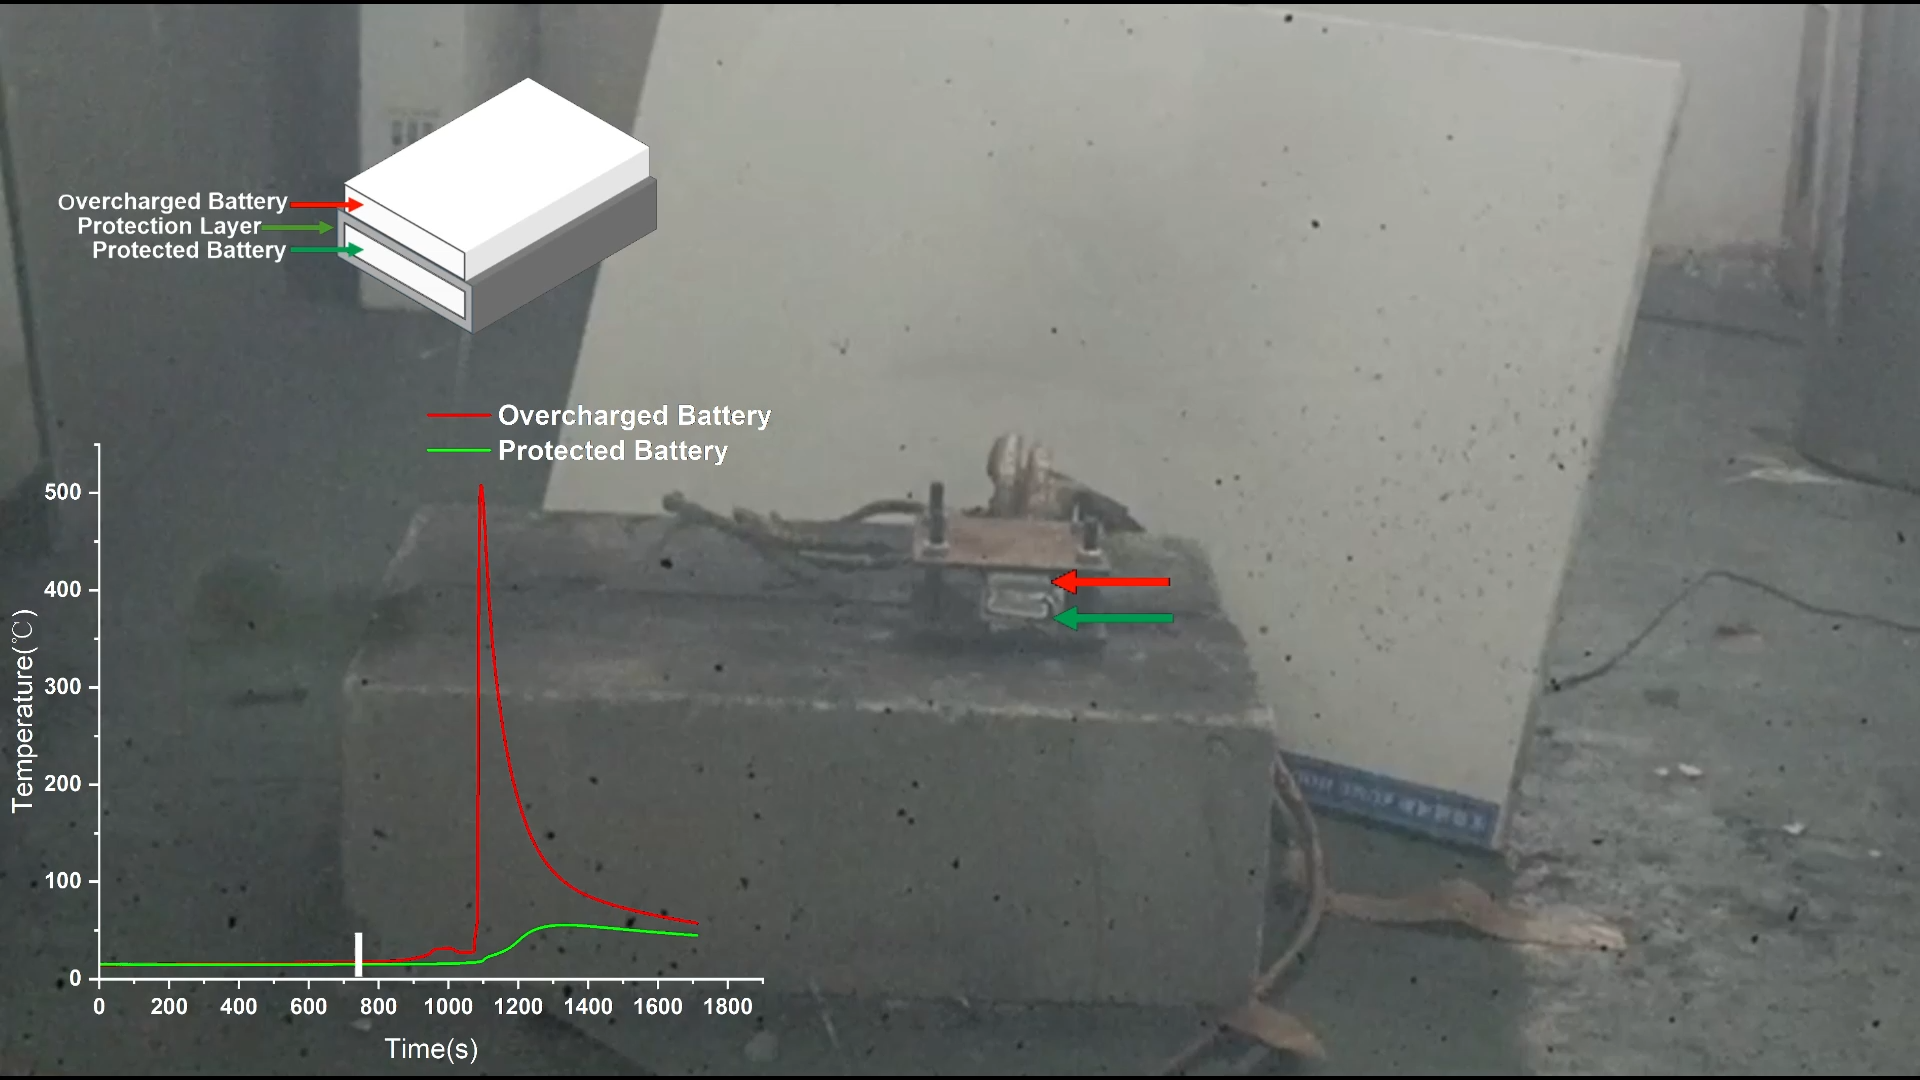
\includegraphics[width=\linewidth]{experiment.png}\\[2pt]
{\scriptsize\color{bsgray} 实景过充测试 —— 起火电芯发生热失控，受保护电芯保持低温。}
\end{minipage}

\vspace{10pt}
\noindent
\begin{tabularx}{\linewidth}{@{}YY@{}}
\toprule
\textbf{过充起火电芯（热失控源）} & \textbf{受保护电池（热盾后侧）} \\
\midrule
峰值温度 \textbf{$>500\,^{\circ}$C} & 峰值温度 \textbf{$<65\,^{\circ}$C} \\
\bottomrule
\end{tabularx}

\vspace{6pt}
\noindent\textbf{结论。} 无火势蔓延、无爆炸，受保护电芯性能几乎未见衰减 —— 满足 GB\,38031-2025
要求。测试流程与结果已获受访头部电池制造商认可，数据来源于实验室公开测试。

% ====================================================== PERFORMANCE
\section{应用带来的整车性能提升}
通过用一层薄材料替代四套子系统，电池热盾释放了电池包体积、提升了热管理裕度 ——
将安全升级同时转化为性能升级。

\vspace{4pt}
\renewcommand{\arraystretch}{1.3}
\begin{tabularx}{\linewidth}{@{}>{\bfseries}p{3.0cm}>{\color{bsgreen}\bfseries}p{2.0cm}Y@{}}
\toprule
\color{bsdark}指标 & \color{bsdark}变化 & \color{bsdark}原因 \\
\midrule
续航里程 & $+$20\,\% & 体积减小，电池包可容纳更多电芯 \\
充电时间 & $-$30\,\% & 更强的热管理支持更高功率充放电 \\
最高速度 & $+$20\,\% & 可承受更高的瞬时放电功率 \\
循环寿命 & $+$20\,\% & 更精确的温度控制延长电池包寿命 \\
\bottomrule
\end{tabularx}

\vspace{6pt}
\noindent\textbf{综合价值：} 满足 GB\,38031-2025、可量化的性能提升与更低的成本 ——
仅占电池包总成本约 10\,\%，远低于现有多系统方案，并帮助电池包厂商以更低保费投保。

% ====================================================== COMPARISON
\section{竞品对比}
\renewcommand{\arraystretch}{1.3}
\footnotesize
\begin{tabularx}{\linewidth}{@{}p{1.9cm}>{\columncolor{bslight}}YYYYYY@{}}
\toprule
\textbf{能力} & \textbf{电池热盾} & 隔热材料 & 灭火系统 & 空冷 & 液冷 & 相变材料 \\
\midrule
被动加热   & \chk & \dash & \dash & \dash & \dash & \dash \\
被动制冷   & \chk & \dash & \dash & 低效 & \dash & 70--110\,J/g \\
热失控延迟 & \textbf{\color{bsgreen}完全阻断} & 5--10\,分钟 & \dash & \dash & \dash & \dash \\
灭火能力   & \chk & \dash & 外围 & \dash & \dash & \dash \\
额外能耗   & \textbf{\color{bsgreen}0\%} & 0\% & \bad{$>$0\%} & \bad{$>$0\%} & \bad{$\sim$5\%} & 0\% \\
体积增加   & \textbf{\color{bsgreen}$<$5\%} & $\sim$5\% & \bad{$>$40\%} & \bad{$>$100\%} & $\sim$20\% & \bad{$>$100\%} \\
成本(占包) & \textbf{\color{bsgreen}总成本$-$30\%} & $\sim$5\% & $\sim$5\% & 0--10\% & $\sim$20\% & \bad{$\sim$50\%} \\
其他风险   & \textbf{\color{bsgreen}无} & \bad{加剧蔓延} & \bad{响应延迟} & \bad{助燃} & \bad{短路风险} & \bad{可燃} \\
\bottomrule
\end{tabularx}
\normalsize
\vspace{2pt}
{\footnotesize\color{bsgray} 数据来源：实验室测试 + 行业专家访谈交叉验证。}

% ====================================================== APPLICATIONS
\section{目标应用场景}
\begin{multicols}{2}
\begin{itemize}
  \item \textbf{新能源汽车} —— 电动汽车、电动卡车、电动船舶
  \item \textbf{低空经济} —— eVTOL 与无人机电池包
  \item \textbf{电网储能} —— 工业级与电网级储能系统
  \item \textbf{可再生能源} —— 光伏、风电配套储能
  \item \textbf{消费电子} —— 手机、笔记本、可穿戴设备
  \item \textbf{智能家居 / 物联网} —— 备用与应急电源
  \item \textbf{医疗设备} —— 生命攸关的电池安全
  \item \textbf{航空航天} —— 卫星与航天器电池包
\end{itemize}
\end{multicols}

\vspace{-4pt}
\noindent\textbf{商业模式。} B2B 供应（标准化产品销售，约占收入 70\%）结合联合开发服务
（针对客户型号的定制设计、认证测试与技术调优，约占 30\%）。目标客户为新能源汽车、
储能与消费电子供应链中的电池包制造商。

% ====================================================== ROADMAP
\section{项目实施计划}
\renewcommand{\arraystretch}{1.3}
\begin{tabularx}{\linewidth}{@{}p{2.8cm}Yp{3.0cm}@{}}
\toprule
\textbf{阶段} & \textbf{主要工作} & \textbf{里程碑} \\
\midrule
\textbf{第 1 年（2026）}\newline 技术验证与中试 &
完成材料配方优化与中试；建立小批量生产线；与 3--5 家头部电池厂技术对接；
完成第三方权威检测认证。 & 技术成熟度达 TRL\,6 \\
\addlinespace[3pt]
\textbf{第 2 年（2027）}\newline 试产与认证 &
建成首条量产线；通过 GB\,38031-2025 国家强制认证；与 10 家以上电池厂签订试用协议；
完成首批客户定点导入。 & 实现首期商业化销售 \\
\addlinespace[3pt]
\textbf{第 3 年（2028）}\newline 规模化与产业化 &
扩大量产规模；进入新能源汽车主流供应链；拓展至储能与消费电子领域；
扩大专利组合。 & 营收突破 5000 万元人民币 \\
\bottomrule
\end{tabularx}

% ====================================================== IP / TEAM
\section{知识产权与团队}
\textbf{知识产权。} 国际 PCT 专利《一种热管理系统》已完成申请；后续将申请中国发明专利，
对配方与制备工艺进行全方位保护，构建专利护城河。

\vspace{4pt}
\noindent\textbf{核心团队与合作。} 一支覆盖材料学、热管理、电池安全与消防工程的多学科交叉团队，
来自\textbf{南洋理工大学（NTU，新加坡）}、\textbf{南京航空航天大学}、
\textbf{哈尔滨工业大学（威海）}与\textbf{慕尼黑工业大学（TUM）}。

\vspace{14pt}
\hrule
\vspace{6pt}
{\footnotesize\color{bsgray}\textit{免责声明：} 本文档中的数据（成本、体积、续航/充电/寿命提升、
$>$500\,$^{\circ}$C 对比 $<$65\,$^{\circ}$C、70 余家访谈及市场预估）来源于项目内部商业计划书、
实验室公开测试数据与行业专家访谈，为指示性数据，最终以独立第三方权威认证为准。
“GB\,38031”指中国电动汽车动力电池安全国家标准。}

\end{document}
